\begin{elevator}[Basic Definitions]	
A \emph{graph} is a mathematical representation of network. We will explore some basic combinatorial properties of graphs, such as paths and cycles. Here, you can also find the definitions of some commonly used graphs like trees and complete graphs. 
\end{elevator}%
\label{sec:graph:basic}% 
Graph theory is a branch of mathematics that naturally arises when you study a group of objects and a relationship that exists between pairs of objects.
For example, you might be studying a group at a party, and the friendships that exist between pairs of attendees.
Even this simple setting presents itself with some interesting questions, like how tight-knit this group is, or which folks at the party are the least related.
Since this type of structure shows up so frequently in mathematics, we will set up an abstract mathematical object called a graph which contains the mathematical data to describe these types of relationships.
\begin{definition}[Graph]
	A \emph{graph} $G$ is a collection of \emph{vertices} $V(G)$ and a set of \emph{edges} 
	\[E(G)\subset V\times V.\]
	The edge is required to be unordered in the sense that  whenever $(v,  w)\in E(G)$,  the pair  $(w,  v)\not\in E(G)$.
\end{definition}
In the case where the graph $G$ is clear, we will suppress the label and simply denote the vertices  by $V$ and edges by $E$.
\nomenclature{$G$}{A graph}
\nomenclature{$E(G)$}{The edge set of a graph $G$}
\nomenclature{$V(G)$}{The vertex set of a graph $G$}
While this definition gives us the mathematical rigor necessary to begin our explanation of graphs, it is useful to have some good examples in mind to ground our discussion.
%\footnote{I usually have a hard time understanding definitions in mathematics without first drawing a picture. In fact, I suggest that on a first reading of this book to look at the pictures before reading the definitions or proofs.}
\begin{examplefigureenv}[Friends in the Order]{191figures/topgraph_potter.tikz}
Let us look at the motivating discussion of groups of friends at a party, and see how this fits into the definition of a graph.
Each person in the population would represent a vertex, and the edges between vertices correspond to the pairs of attendees who are friends.
\end{examplefigureenv}
\begin{framedpage}{example}{Some Common Graphs}{It is good to have some examples of graphs in mind before we go around discussing the theory of graphs.}

\begin{smallexamplefigureenv}[Graph:]{191figures/topgraph_graph.tikz}
One way to construct a graph is to build it by hand. 
For example, we can give a graph four vertices and 4 edges by specifying
  \[V=\{1,2,3,4\}\;\;\; E=\{12,23,13,14\}.\]
 While mathematically precise, this presentation is not very intuitive, and so when we want to specify a graph in this text, we will usually just draw a picture of that graph, and assume that it has some explicit (although unwritten) labeling of the vertices and edges.
\end{smallexamplefigureenv}


\begin{smallexamplefigureenv}[Complete Graph:]{191figures/topgraph_completegraph.tikz}
  One especially important family of graphs are the \emph{complete graphs}, which are saturated with edges.
\noindent Let $n\in \N$ be a natural number. The \emph{complete graph on $n$ vertices},  denoted as $K_n$, is the graph with $n$ vertices and an edge between every pair of vertices. 
Since every edge corresponds to a choice of 2 vertices, and in the complete graph we've chosen every pair, it follows that 
\[|E_{K_n}|={n\choose 2}.\]
One reason we call this graph complete is because every graph on fewer than $n$ vertices is a subgraph of $K_n$. 
\end{smallexamplefigureenv}
\nomenclature{$K_n$}{The complete graph with $n$ vertices}


\begin{smallexamplefigureenv}[Octahedron:]{191figures/topgraph_octahedron.tikz}
Graphs naturally arise from other branches of mathematics. 
For example, every polyhedra in $\RR^3$ determines a graph by its edges and vertices. In the diagram on the left, we see the graph corresponding to the octahedron.
Later, we will classify the platonic solids by understanding the combinatorics of their corresponding graphs. 
Notice that a polyhedron has more data than just its underlying graph, as it also knows what combinations of edges and vertices make up faces of the polyhedron. 
\end{smallexamplefigureenv}
\end{framedpage}
A good way to understand a graph is to draw a diagram of it, by placing a  dot for each of the vertices, and drawing a line segment or curve between two vertices if that pair is inside of the edge set $E$. 
The edges of these diagrams are allowed to cross each other, and the edges need not be drawn straight.

Even after introducing a couple of graphs, we can already see some interesting topological properties.
For instance, the complete graph on 5 vertices can only be drawn with edges that cross, whereas every graph that represents a platonic solid can be given by a planar drawing without edges crossing.
Before we get to describing topological properties of graph, let's first describe some of the combinatorial data attached to a graph. 

In this text, the vertices of a graph will be labelled with lowercase letters $u, v, w, x, y.$
For edge, we will either use the letters $e, f$; or we will refer to an edge with endpoints $u$ and $v$ by the pair $uv$. With this notation, we say that $uv$ is an edge if either $(u, v)\in E$ or $(v, u)\in E$. 
\nomenclature{$N(v)$}{The neighborhood of a vertex $v$}
The simplest piece of data that we can ask about a vertex in a graph is the number of neighbors it has.  
\begin{definitionfigureenv}[Neighborhood]{191figures/topgraph_neighborhood.tikz}
	Fix some vertex $v$. Then the subset of vertices which are connected to $v$ by an edge is called the \emph{neighborhood} of $v$, and will be denoted 
	\[N(v):=\{u\in V \;|\; (u,v) \text{ or } (v, u)\in E\}\]
	 The number of edges connected to $v$ is called the \emph{degree} of $v$ and is denoted 
	\[\deg(v):=|\{u \in N(v)\}|.\]
\end{definitionfigureenv}

\nomenclature{$\deg(v)$}{The degree of $v$}
We can already capture a lot of data about a graph simply by knowing the degrees of the vertices in it.
For example, if $|V(G)|=n$, and every vertex has degree $|n-1|$, then it must be the case that $G=K_n$.
If instead every vertex has degree 2, then it must be the case that $G$ is a collection of cycles.
Both of these give us example of  \emph{regular graphs}, which are graphs whose vertices all have the same degree.
A natural family of regular graphs that show up are the Platonic solids.

The degree of a vertex provides \emph{local} information about the graph.
This means that knowing the degree of a particular vertex $v\in G$ doesn't tell us a lot about the graph as a whole --- we only learn about a small portion of the graph around $v$.
This is contrasted with quantities like $|E(G)|$ and $|V(G)|$, which tell us \emph{global} information about our graph. 
In many ways, topology is the study of how local information can be meaningfully assembled into global data. 
\begin{claim}[Average vertex degree]
Let $d(G)$ be the average degree of the vertices of a graph.
The total number of edges in $G$ is:
\[2|E|=d(G)|V|.\]
\label{claim:avgdegree}
\end{claim}
Here, we are using averaging to take local information -- the degree -- and obtaining some information about the entire graph. 
The rough idea of proof is that every edge contributes $+1$ to the degree of each of its ends, so that the sum of all the degrees of the vertices will be twice the number of edges. 
We therefore obtain the equality 
\[2|E|= \sum_{v\in V} \deg(V)= d(G)|V|.\]

But let's try to make this argument a little more mathematically watertight.
%\footnote{As with many mathematical proofs, the outline of the proof is much easier to comprehend than the detailed exposition.
%If you're reading this for the first time, feel free to look at pictures and skip the detailed expositions if you've gotten the gist of the proof.
%Sometimes reading the details just makes the idea of the proof more muddy due to the need to unpack definitions and use notation.}  
\begin{proof}
	From the definition of average degree 
\begin{align*}
d(G)|V|=&\sum_{v\in V}\deg (v)
=\sum_{v\in V} \sum_{u\in V} \delta_E(u,v)+\delta(v, u)
\intertext{where $\delta_E(u,v)=1$ if $(u,v)\in E$, and 0 otherwise. The reason both orders are necessary is because our definition of edge used ordered pairs $(u,v)$.}
=&\sum_{(u,v)\in V\times V} \delta_E(u, v)+\delta_E(v, u)
\intertext{As $\delta(u, v)$ only takes a value of 1 on sets $(u, v)$ that are in $E$, this term counts the number of edges}
=& 2|E|
\end{align*} 
\end{proof}
A good example keep in mind for this lemma are the complete graphs. These $n$-vertices of these graphs each have $(n-1)$ neighbors, so by \sref{claim:avgdegree}  the number of edges in a complete graph is $\frac{n(n-1)}{2}$. 
We also get this strange, but surprisingly useful, corollary. 
\begin{corollary}[An Even number of odd vertices]
	The number of odd degree vertices in any graph is even. 
\end{corollary}
The proof is left to  \sref{exer:evengraph}.
One general mathematical principle is that a large, complicated object (like a graph) can be understood by asking questions about its substructures. 
For instance, by asking how many edges or how many vertices are in a graph, we can begin to get an understanding of its global structure.
In the setting of graphs a particularly useful substructure to study are subsets of the edges and vertices which themselves make \emph{subgraphs} of $G$.
Here are two especially important types of subgraphs which we will look at throughout the course.

\begin{definition}[Paths and Cycles]
	Let $G$ be a graph. A \emph{path} in $G$ is a sequence of distinct vertices $\{v_i\}_{i=0}^n$ such that $v_iv_{i+1}$ is an edge in $G$ for every $i$. The length of the path is the number of edges in it. We say that a path \emph{starts at $v_0$ and ends at $v_k$.} A \emph{cycle} in $G$ is a path $P$ such that the first and last vertex of $P$ share a common edge (which is not already in the path $P$)% \footnote{A word of caution for those who may be using another text; there is some disagreement about whether paths are allowed to repeat vertices or edges. You may see variations of the above definition being called a simple path, or trail, or walk, depending on where you look.}
\end{definition}

Paths and cycles are useful subgraphs to study as they can probe \emph{global} data about the graph.
If you know that a graph has a path between any two points, or that a graph contains no cycles, then you've learned something interesting about the global topological information of that graph.

\begin{examplefigureenv}[Paths and Cycles]{191figures/topgraph_cycle.tikz}
 In the drawn example, we have a path 4 highlighted in red, and a cycle of length 3 highlighted in blue.
The longest path that one can draw would have length 5, and the largest cycle has length 6. 
\end{examplefigureenv}
Since every edge constitutes a very short path, it will necessarily be the case that a non-trivial graph has some paths in it.
However, it need not be the case that a graph have any cycles.
\begin{examplefigureenv}[Trees]{191figures/topgraph_tree.tikz}
	A \emph{tree} is a graph with a unique path between any 2 points. 
	This is a global property of a graph.
	If we fix a vertex $v$ in the tree (called a root), then the set of paths that start at $v$ are in bijection with the vertices in the tree.
	In \sref{exer:tree}, several different interesting properties of a graph are shown to be equivalent to being a tree. 
\end{examplefigureenv}
The length of the longest path in a graph $G$ is telling us something about the global structure of the graph-- you need to look at the entire graph to find the longest path.
As before, we look at how we can assemble local information -- in this case, the degrees of the vertices -- to provide some information on this invariant.
\begin{claim}
	Let $\delta$ be the minimal degree of the vertices in $G$. Then $G$ has a path of length $\delta$. 
\end{claim}	
\begin{proof}
	Start with any path $P$.
	% \smarginnotel{\margingraphics{191figures/topgraph_minpath}} 
	Let $\{v_i\}$ be the vertices of the path.
	Let's look at initial vertex of the path , $v_0$. 
	Suppose that we can find a vertex $w\in N(v)$, which is not already contained within the path $P$. 
	Take this vertex $w$, and append it onto $P$ to build a new path $wP$ which is one vertex longer.

	We can continue this process unless we've grown our initial path to a path  $P'$ which can no longer be extended. This will happen if every point in the neighborhood of the end of the path is contained within the path.  
	For this path $P'$, we have $N(v_0)\subset V(P')$.
	Since $\delta \leq |N(v_0)|<|V(P)|$, we conclude that $\delta \leq |E(P)|$. 
\end{proof}
\begin{elevator}[Connectivity]
	A graph is connected if you can travel between any two vertices along the edges of the graph. We also look at several different quantitative measurements of connectivity.
\end{elevator}
\label{sec:graph:connectivity}
Topology is the study of mathematical structures which have a notion of how their parts are connected to each other.
A graph is an example of a topological structure, as each vertex ``knows'' which neighbors it is connected to. 
By travelling from vertex to vertex along edges, we can explore questions about the global connectivity of a graph.

\begin{definitionfigureenv}[Vertex Connectedness]{191figures/topgraph_disconnectingset.tikz}
	A graph $G$ is called \emph{connected} if for any two vertices $v$ and $w$,  there exists a path from $v$ to $w$. 
	A disconnecting set $U\subset V$ is a set of vertices with the property that the graph $G\setminus U$ is disconnected.
	The \emph{connectivity of $G$}, denoted $\kappa(G)$, is the size of the smallest disconnecting set of $G$.  
\end{definitionfigureenv}

The connectivity of a graph is an important measurement for applications.
For example, if we are building a power grid for a utility, then whether or not the power can be delivered to the entire network from a single node is determined by the connectedness of the underlying graph. 
The connectivity of the network is a slightly stronger measure, which tells us the maximal number of nodes of the network can fail and still have the network remain connected.
We have a property of a graph which interpolates between the connectivity number and the connected property. We say that a graph is $k$-connected if no vertex set of size $k$ disconnects the graph $G$.
Equivalently, a graph is $k$-connected if its connectivity is at least $k$. 

%\begin{figure}
%	\centering
%	
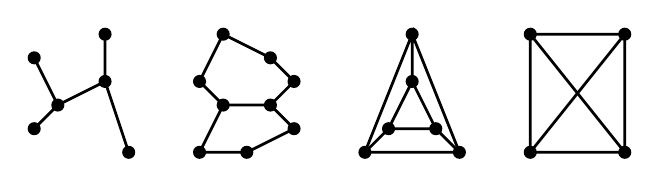
\begin{tikzpicture}[scale=.3]
    \newcommand{\vertexradius}{2.5pt}
\newcommand{\vertexscale}{.5}
\newcommand{\bigvertexscale}{1}
\newcommand{\vertex}{\node[circle, fill=black, scale=\vertexscale] }
\newcommand{\highlighta}{red!20}
\newcommand{\highlightb}{blue!20}
\newcommand{\highlightc}{green!20}
\newcommand{\shadinga}{gray!20}
\newcommand{\smallvertex}{\node[circle, fill=black, scale=.2]}
\newcommand{\highlightlinewidth}{3pt}

\tikzset{every path/.style={line width=1 pt}}
\vertex at  (14,5){};
\vertex at  (9,1) {};
\vertex at  (7,0) {};
\vertex at  (5,0) {};
\vertex at  (9,3) {};
\vertex at  (8,4) {};
\vertex at  (8,2) {};
\vertex at  (6,2) {};
\vertex at  (5,3) {};
\vertex at  (6,5) {};
\vertex at  (2,0) {};
\vertex at  (-2,1){};
\vertex at  (1,3) {};
\vertex at  (-1,2){};
\vertex at  (1,5) {};
\vertex at  (-2,4){};
\vertex at  (23,5){};
\vertex at  (23,0){};
\vertex at  (19,5){};
\vertex at  (19,0){};
\vertex at  (16,0){};
\vertex at  (15,1){};
\vertex at  (14,3){};
\vertex at  (13,1){};
\vertex at  (12,0){};
\draw (1,5) -- (1,3)  -- (2,0);
\draw (-2,1) -- (-1,2) -- (-2,4);
\draw (-1,2) -- (1,3);
\draw (6,5) -- (5,3) -- (6,2) -- (8,2) -- (9,3) -- (8,4) -- (6,5);
\draw (6,2) -- (5,0) -- (7,0) -- (9,1) -- (8,2);
\draw (14,3) -- (13,1) -- (15,1) -- (14,3);
\draw (14,3) -- (14,5) -- (12,0) -- (16,0) -- (14,5);
\draw (12,0) -- (13,1);
\draw (15,1) -- (16,0);
\draw (19,5)  -- (19,0) -- (23,0) -- (23,5) -- (19,5) -- (23,0);
\draw (19,0) -- (23,5);
\pgfsize \end{tikzpicture}


%	\caption{Graphs with connectivity 1, 2, 3, and 4. }
%\end{figure} 


\begin{examplefigureenv}[Bottlenecks and Connectivity]{191figures/topgraph_risk.tikz}
	If $H\subset G$ is a subgraph, one can measure the size of the smallest set it takes to disconnect $H$ from the remainder of $G$.
	This will always be at least the connectivity of the entire graph.
	In the game of \emph{Risk}, the continent of Australia is especially prized because of it's low vertex connectivity to the remainder of the graph. 
\end{examplefigureenv}

\nomenclature{$\kappa(G)$}{The vertex connectivity of $G$}
Connectivity has a strange relationship with topology.
Whether or not a graph is connected is a \emph{topological} property of the graph. However, the connectivity of a graph is \emph{not} a topological property.
An example that demonstrates that connectivity is not a topological property are the graphs of the triangle and the square, which are topologically indistinguishable.
However, the triangle is three connected, and the square is only 2 connected! We will later see in \sref{sec:graph:Minors} exactly why connectivity is not a topological property. 
You can observe that even making small modifications to the graph (like making the edge of a graph into a path,) can greatly change to the connectivity of a graph. 

It is possible to get an estimate on the connectedness of an average component of the graph by knowing the average degree of the vertices of a graph.
In short, if you have a lot of edges, then we expect the graph have a connected component with high connectivity (see \sref{graph:thm:mader}.)


\begin{framedpage}{theorem}{Mader's Theorem}{Every graph with average vertex degree $d(g)$ greater than $4k$ contains a $k$-connected subgraph. \label{graph:thm:mader}}
	The idea of this proof is to induct on the number of vertices, where the vertex we remove during the inductive step is one of low degree. We start by massaging $d(G)\geq 4k$ to obtain the inequalities
	\begin{align*}|V|\geq 2k-1 && |E|\geq (2k-3)(|V|-k+1)+1\end{align*}
	For the first inequality, notice that if the average degree is $4k$, there must be a vertex with degree at least $4k$; therefore it has $4k$ neighbors. Therefore the number of vertices is at least $4k$. 
	For the second inequality, we apply \sref{claim:avgdegree},
	\[|E|= d(G)|V| \geq  4k  |V| 
	\geq(2k-3)(|V|-k+1)+1\]
	With these two new inequalities, we run an inductive argument on the number of vertices in the graph. In the base case, $G$ is a graph on $2k-1$ vertices and therefore is complete, for which the claim follows trivially.

    For the inductive step, we split into two cases based on whether there exists a vertex of low-degree. If $v$ has low degree, then $G\setminus v$ will have \emph{larger}  average degree, and by induction we can still run our argument. 
    
	\textbf{Case 1:} Suppose that there exists a vertex of degree less than $2k-3$. Then even after removing this vertex, our inductive hypothesis holds as we've decreased the number of vertices by 1 but only removed at most $(2k-3)$ edges.
\begin{paragraphfigureenv}[]{191figures/topgraph_disconnect.tikz} 
	\textbf{Case 2:} Suppose that the inequality is not sharp,  and we cannot find a vertex of degree $2k-3$ or less. Let's assume for contradiction that $G$ is not $k$-connected. Then there are two subgraphs $G_1,  G_2\subset G$ such that $G_1\cap G_2$ has fewer than $k$ vertices. 
	Every vertex in $G_1\setminus G_2$ has neighbors only in $G_1$. Since the minimal degree of each vertex is $2k-2$,  we have that $G_1$ has at least $2k-1$ vertices. Similarly,  $G_2$ has $2k-1$ vertices. So, both the graphs $G_i$ satisfy the first inequality for our induction hypothesis.
	\end{paragraphfigureenv} As $E=E_1\cup E_2$, we get $|E|\leq |E_1|+|E_2|$. We additionally know that $|V_1|+|V_2|\leq |V|+k$. Combining these inequalities gives
	\[(2k-3)(|V_1|-k+1)+1)+(2k-3)(|V_2|)-k+1)\leq (2k-3)(|V|-k+1)+1\leq |E|\leq |E_1|+|E_2|\]
	from which we conclude that one of the $G_i$ satisfy the induction hypothesis, and therefore contains a $k$-connected subgraph. 
\end{framedpage}

There is no particular reason why we choose to use deletion of vertices to define the connectivity of a graph. 
We could have instead used edges to get a measure of connectivity, and define the \emph{edge connectivity} as the minimal number of edges that you must remove to disconnect the graph.
Somewhat surprisingly, the vertex connectivity and the edge connectivity are usually not related to each other.
\begin{examplefigureenv}[Dumbbell Graph]{191figures/topgraph_dumbbell.tikz}
Consider the dumbbell graph which is created by taking two $K_n$ and mutually connecting them to a new vertex $v$. 
In order to disconnect this graph by removing edges, you need to remove at least $n$ edges.
However, to vertex disconnect the graph, it suffices to take out the middle vertex $v$.
\label{fig:graph:dumbell}
%See Exercise \sref{exer:edgeconnectivity} for a basic bound. 
\end{examplefigureenv}
The discrepancy between the edge and vertex connectivity is due to the fact that a concentrating edges onto a single vertex gives it low vertex connectivity, but has little impact on edge connectivity.


\begin{projectdescription}{Spectral Graph Theory}
A more quantitative measure of connectivity examines the average distance squared between two vertices in the graph.\label{proj:spectral}
We now give a nice algebraic characterization of this metric. 
Let  $V=\{v_1, \ldots, v_n\}$ be the vertices of a graph $G$. 
The \emph{adjacency matrix of $G$}  is the $n\times n$ matrix $A$ whose $ij$ entry is $1$ if $v_iv_j$ is an edge, and $0$ otherwise.
Define the \emph{degree matrix} $D$ to be the diagonal matrix whose $i$th diagonal entry  is $\deg(v_i)$.
Finally, we define the \emph{Laplacian} of the graph $G$ to be the matrix 
\[
	L=D-A.
\]
The eigenvalues of $L$ bound the connectivity of $G$, and in applications gives a more nuanced definition for connectivity.
\end{projectdescription}

As demonstrated by the dumbbell graph (\sref{fig:graph:dumbbell}), the vertex connectivity tells us where the bottlenecks are in our graph. 
Another way of counting the bottlenecks in a graph would be to ask how many independent paths there are between two vertices, as the presence of a bottleneck in the graph will force this number to be small.
\begin{definition} [$k$-path connected]
	A graph is \emph{$k$-path connected} if any two vertices $v$ and $w$ can be joined by at least $k$ disjoint paths. 
\end{definition}
You can check that  the dumbbell graph (\sref{fig:graph:dumbbell}) is only 1-path connected, as there is only one way to get from the left portion of the graph to the right portion. Menger's theorem (\sref{graph:thm:mengers}) tells us that this is generally the case: the path connectivity of a graph is equal to its vertex connectivity.

Menger's theorem seems a bit strange on first reading because of a contrast in the definition of path connectedness and vertex connectedness. 
The path connectivity looks to  \emph{maximize} a set of independent paths, while the vertex connectivity is tries to  \emph{minimize} the size of a disconnecting set.

\begin{projectdescription}{Max-Min}
These types of statements are common in combinatorics related to optimization.
Max-Min properties extend to many combinatorial  \label{proj:maxmin}  objects beyond graphs,  and the Max-Min principle has several statements which are all relevant to optimization of networks.  Some equivalent theorems to Menger's theorem include the Max-flow Min-cut theorem, K\"onig's theorem, Dilworth's theorem, and Hall's theorem.
\end{projectdescription}


One application of Menger's theorem is to classify the structure of graphs with connectivity $2$.
\begin{lemma}[Adding paths preserves $\kappa(G)\geq 2$]
	Suppose that $\kappa(G)\geq 2$.
	 Let $v,w$ be two vertices in $G$. 
	Create a new graph, $G\cup_{v,w} P$ by attaching a path of length at to $G$, whose endpoints are $v$ and $w$. 
	Then $\kappa(G\cup_{v, w}P)\geq 2$.\\
	If additionally we require that the path have at least 3 vertices, then $\kappa(G\cup_{v, w}P)=2$. 
\end{lemma}
\begin{proof}
	Suppose for contradiction that $\kappa(G\cup_{v, w}P)=1$. Then there is a disconnecting vertex $u$ so that $G\cup_{v, w}P\setminus \{u\}$ is disconnected.
	It must be the case that $u\in P$, as otherwise $G\setminus \{u\}$ would be disconnected, contradicting that the 2-connectivity of $G$. 
	If $P$ has only two vertices, $\{v, w\}$ we are done (as every candidate vertex for $u$ needs to lie outside of $G$, but $V(G\cup_{w,v}P)=G(P)$. Therefore the length of $P$ must be at least 2. The removal of $u$ from  $P$ separates the path into two 2 components. 
	Each of those components is connected to $G$ by their ends, and therefore $G\cup_{w,v}P\setminus\{u\}$ is still connected.
	$u$ fails to be a disconnecting vertex for $G\cup_{w,v}P$, contradicting our assumption. 

	It remains to show that if the length of $P$ is at least 2, that there exists a disconnecting set for $G\cup_{w,v}P$ of size 2. Observe that $G\cup_{w,v}P\setminus\{w, v\}$ is disconnected if there are any vertices in $P$ besides $w$ or $v$. 
\end{proof}

\begin{doubledpage}{theorem}{Menger's Theorem}{
	The path connectivity of a graph is equal to the vertex connectivity of the graph.  }
\label{graph:thm:mengers}
We first show that the path connectedness is at most the vertex connectedness. 
Suppose that  $v_1, \ldots, v_k$ form a disconnecting set which separates $G$ into two components $G_1$ and $G_2$.
Pick a vertex $u_1\in G_1$, and $u_2\in G_2$.
There can be at most $k$ disjoint paths between $u_1$ and $u_2$, as each path must use one of the $k$ points in the intersection.
This shows that the path connectivity is less than the vertex connectivity.
\begin{paragraphfigureenv}[Setup:]{191figures/topgraph_mengersetup.tikz} To show that the path connectedness is at least the vertex-connectedness, we will prove a stronger statement.  Suppose that $G$ is $k$-connected,  and let $A$ and $B$ be disjoint subgraphs of $G$.
We will show that whenever we have a collection of fewer than $k$ disjoint paths from $A$ to $B$, we can find a larger connection of disjoint paths from $A$ to $B$. Let's set up some notation for this. 
\end{paragraphfigureenv}
\begin{claimfigureenv}[Inductive statement for Menger's Thm.]{191figures/topgraph_mengersetup2.tikz}
Suppose that $A$ and $B$ are subgraphs of $G$ each containing at least $k$ vertices.
Let $b_1, \ldots, b_n$ be vertices of $B$, with $n<k$. 
Let $\mathcal P_n=\{P_1, \ldots , P_n\}$ be a collection of disjoint paths $G$, which 
\begin{itemize}
    \item only intersect $A$ at their left endpoints,
    \item only intersect $B$ at their right endpoints, which are the specified vertices $b_i$. 
\end{itemize}
Then there exists a point $y\in B$ and  collection $\mathcal P_{n+1}$ of $n+1$ disjoint paths in  $G\setminus (A\cup B))$ which satisfy the above conditions, with right endpoints $b_1, \ldots, b_n, y$. 
\end{claimfigureenv}

We will prove this by inducting  on the size of $G\setminus B$. When $B$ is all of $G\setminus A$, then each path $P_i$ consists of a single edge, and $k$-connectedness gaurentees that $A$ cannot be separated from $B$ by fewer than the removal of $k$-vertices.
For our inductive step, let us assume that the claim holds for every subgraph $B'$ containing $B$.  Let's look at our current graph and subgraph $B$. 
Now, we will randomly construct a new path $Q$ from $A$ with a  random endpoint in $B$.
If this path is disjoint from the $\mathcal P_n$, then we are done.
Now, we use the inductive hypothesis by expanding the subgraph $B$ to include a point from the path $Q$. Let $x$ be the final point where the path $Q$ intersects the collection $\mathcal P_n$, and without loss of generality we will assume that $x$ lies on the path $P_n$.
\begin{paragraphfigureenv}{191figures/topgraph_mengersetup3.tikz}
     Denote by $Q_y$ the segment of $Q$ going from $x$ to $y$, and $Q_b$ the segment of $Q$ going from $x$ to $b_n$.  Now  enlarge $B$ by including the path $Q_b$ and $Q_y$, 
\[B':= B\cup Q_b\cup Q_y.\]
The end points $b_1, \ldots, b_{n-1}, x$ satisfy the conditions of the claim.  By our inductive hypothesis, there exist disjoint paths $\mathcal P_{n+1}'$ going from $A$ to end points $b_1, \ldots, b_{n-1}, x, z$ in $B'$. 
\end{paragraphfigureenv}

At this point we've found a subgraph $B'$ containing $B$, and we would like to reduce down to $B$.
We break into different cases based on the location of the point $z$. 

\begin{paragraphfigureenv}{191figures/topgraph_mengercase1.tikz}
    \textbf{Case 1:} In the easy case, $z$ belongs to our original set $B$. In this case, replace $y$ by $z$ in the original step. The paths $P_1', \ldots P_{n-1}'$ and $P_{n+1}'$ with endpoints $b_1, \ldots, b_{n-1}, z$ are disjoint. To create a final path with endpoint on $b_n$, we take the concatenation of the path $P_{n}'$ with endpoint $x$, and the path $Q_b$. Since $Q_b\subset B'$, it is disjoint from all of the $P'_i$ we've constructed so far. This gives us the collection $\mathcal P_{n+1}$ 
\end{paragraphfigureenv}
The more difficult case is when  $z$ only belongs to the enlargement  $B'$. Then $z\in B'\setminus B = Q_b\sqcup Q_y$. By construction, the paths $Q_b$ and $Q_y$ are disjoint, so either $z\in Q_b$ or $z\in Q_y$. 
\begin{paragraphfigureenv}{191figures/topgraph_mengercase2.tikz} \textbf{Case 2a}
    Suppose that $z\in Q_y$. Then consider the paths 
    \begin{itemize}
        \item $P''_n$, which is $P'_n$ concatenated with $Q_b$, and 
        \item $P''_{n+1}$, which is $P'_{n+1}$ concatenated with the portion of $Q_y$ lying after $z$. 
    \end{itemize} 
    These two paths are disjoint from the $P'_1, \ldots, P'_{n-1}$, and are additionally disjoint for eachother. These paths are seen to have interior vertices which are disjoint from $B$, and by construction have left endpoints in $A$. The $\{P_1', \ldots, P'_{n-1}, P''_n, P''_{n+1}\}$ satisfy the conditions of the claim. 
\end{paragraphfigureenv}

\begin{paragraphfigureenv}{191figures/topgraph_mengercase3.tikz}
    \textbf{Case 2b}
     Alternatively, it may be the case that $z$ lies on the path $Q_b$. T
     \begin{itemize}
         \item $P''_n$, which is $P'_{n+1}$ concatenated with $Q_b$, and 
         \item $P''_{n+1}$, which is $P'_{n}$ concatenated with the portion of $Q_y$ lying after $z$. 
     \end{itemize}  
     As in the previous case, the paths $\{P_1', \ldots, P'_{n-1}, P''_n, P''_{n+1}\}$ satisfy the conditions of the claim.
\end{paragraphfigureenv} 
\end{doubledpage}
This gives us a method to build larger 2-connected graphs from smaller 2-connected graphs.
This can be strengthened to a characterization of $2$-connected graphs. 
\begin{theorem}[Characterization of 2-connected graphs]
	Let $G$ be a 2-connected graph. Then either 
		\begin{itemize}
			\item 
			There is a 2-connected graph $H$ so that $G$ may be obtained by attaching a path of $H$ and
			\[G=H\cup_{v,w} P.\]
			\item 
			$G$ is a cycle.
		\end{itemize} 
\end{theorem}
\begin{proof}
	Suppose that $G$ is not a cycle.
	Since $G$ is 2-connected, $G$ contains at least a cycle.
	This means that $G$ contains a 2-connected subgraph, and so we can find a maximal 2-connected proper subgraph $H$. 
	Here, maximal means that there does not exist another proper 2-connected subgraph $H'$ containing $H$. 
	We would like to show that $G$ is obtained by attaching a path onto the graph $H$. 


	Look at a vertex $v\in G\setminus H$, and a vertex $w\in H$.
	As $G$ is 2-connected,  Menger's theorem ensures that there exists disjoint paths $P_1, P_2$ from $v$ to $w$.
	This gives two paths from $w$ to that are contained in $H$.
	$H\cup P$ is a 2-connected subgraph of $G$.
	It cannot be the case that $H\cup P$ is a proper subgraph, because $H$ was assumed to be the maximal proper 2-connected subgraph of $G$.
	It must then be the case that $G=H\cup P$, concluding the proof. 
\end{proof}
This gives us way to build up all 2-connected graphs. 
\begin{corollary}
	Every 2-connected graph is generated from a cycle with the subsequent addition of paths.
\end{corollary}
We will have to develop a few more tools before we're able to get  a classification result for 3 connected graphs, and will return to this in \sref{sec:graph:3connected}.

